\section{Subtype}
\begin{enumerate}
	\item[1)]
	Vi opskriver koden for en 4-bit subtractor som ses i kode \ref{lst:SubtractorCode}
	\begin{lstlisting}[caption={Subtractor kode},label={lst:SubtractorCode}]
	library ieee;
	use ieee.std_logic_1164.all;
	
	entity Subtypes is
	port (a,b : in std_logic;
	c  : out std_logic);
	end Subtypes;
	
	architecture dataflow of Subtypes is
	subtype bool is std_logic range '1' to 'Z';
	signal tmp : bool;
	begin 
	tmp<= 'U';
	c<= b and tmp;
	end dataflow;
		\end{lstlisting}
	\item[2)]
	
	Grunden til at vi får fejlen at U er udenfor rækkevidde ses på figur \ref{fig:stdulogicvalues} nedenfor:
	
		\begin{figure}[H]
			\centering
			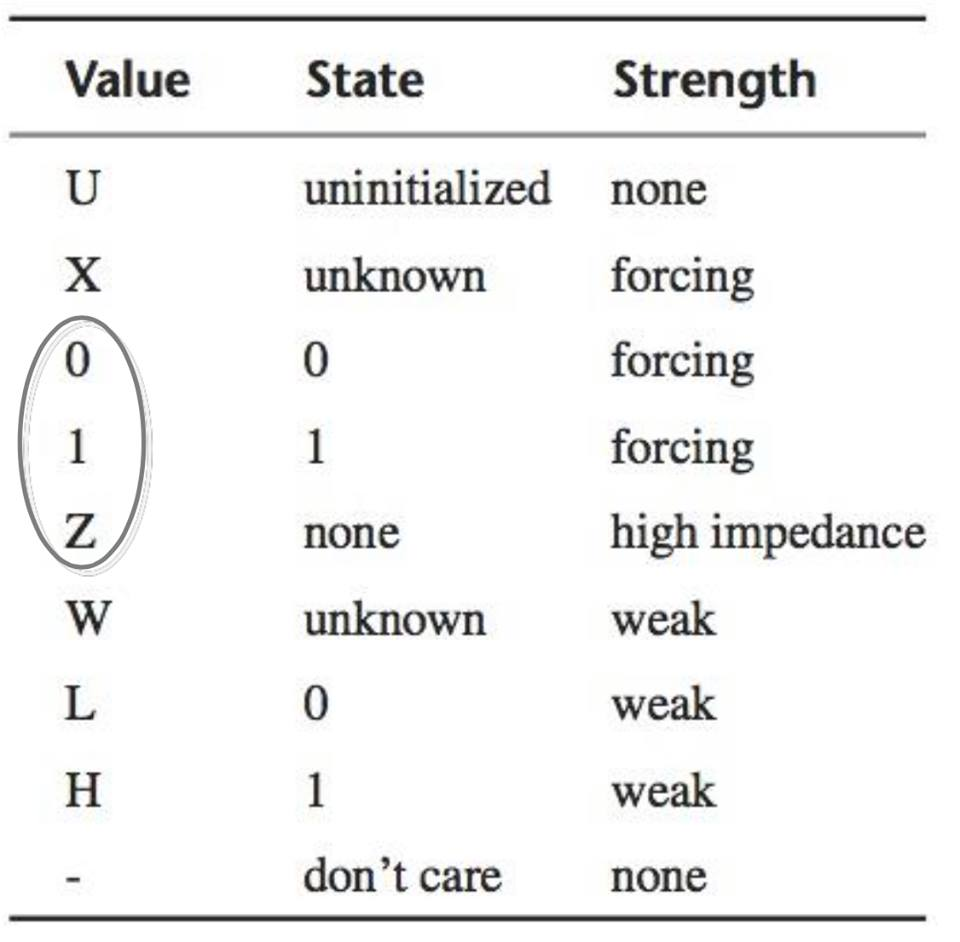
\includegraphics[scale=0.23]{pictures/Oevelse3/Oevelse4_01Z.jpg}
			\caption{Stater og styrker for std\_ulogic værdier}
			\label{fig:stdulogicvalues}
		\end{figure}
	
	
	Derfor retter vi til koden
	
	\begin{lstlisting}[caption={Rettet subtractor kode},label={lst:SubtractorCode2}]
library ieee;
use ieee.std_logic_1164.all;

entity Subtypes is
port (a,b : in std_logic;
c  : out std_logic);
end Subtypes;

architecture dataflow of Subtypes is
subtype bool is std_logic range 'U' to 'Z';
signal tmp : bool;
begin 
tmp<= 'U';
c<= b and tmp;
end dataflow;
	\end{lstlisting}	

	
\end{enumerate}


